{Create a function called \cour{plotlines} with two inputs and no outputs with the following details.  The first input should be a $1 \times 2$ matrix (representing the base point, B, in the plane).  The second input should be a $2 \times 2$ matrix (representing two more points in the plane, P and Q).  When the function is run, there should be a plot of two line segments, BP and BQ, with the two distances displayed halfway along each line.}
{}
%For example:\\
%\cour{>> plotlines([1, 1],[2, 4;5, 6])}\\
%would give\\
%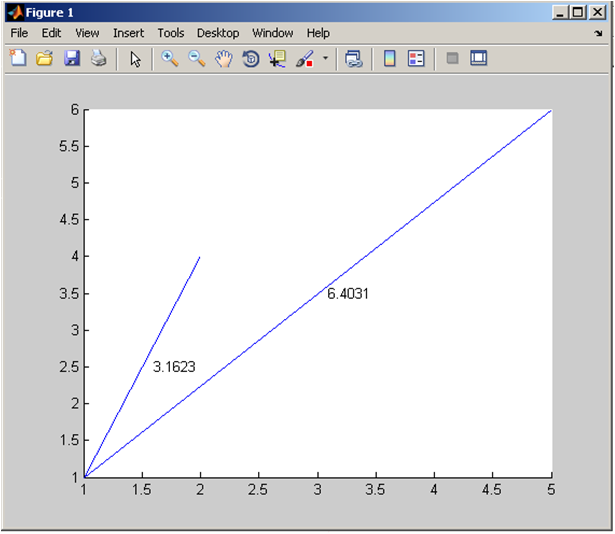
\includegraphics[scale=.6]{figures/matlab_functionplot1.png}}

